We used adaptive dynamics theory to study the conditions favorable to parapatric adaptive speciation in a sexual, diploid species spread across two patches. 

% Selection determines whether branching occurs

The strength of divergent selection is an important parameter in determining whether branching will occur. Whether selection is needed to trigger branching depends on environmental heterogeneity. When the landscape is homogeneous (habitat symmetry  is $1$), a minimal amount of selection is needed for branching to occur (Fig. \ref{fig:map_branching_points}). This minimum amount is a selection coefficient value of $s = 0.5$, which is the point at which the reproductive success function $W$ (proportional to the sum of the two attack rate functions in Fig. \ref{fig:attack_rates} in a homogeneous environment) goes from being unimodal to being bimodal, thus producing two peaks in the adaptive landcape. For $s > 0.5$, specialists i.e. individuals with trait values closer to $\pm 1$, have a higher payoff than generalists i.e. individuals with trait values closer to zero. Although a two-peaked fitness landscape imposed by the resources would in itself favor the splitting of a population only if this population is sitting at the bottom of the valley between the two hills, branching can occur even when starting with a specialist population (e.g. with initial trait value $x = -1$ in Fig. \ref{fig:map_branching_points}) because of disruptive frequency-dependent selection arising as a result of competition. This case is analogous to the classical sympatric speciation scenario.\\

% Selection less needed when habitat asymmetry is higher

On the contrary, when habitat heterogeneity increases, divergent selection may be less, or not at all, needed for branching. This is because as habitat asymmetry increases, one resource becomes more abundant and more advantageous to exploit in one of the two habitats, while the other resource becomes more advantageous in the other habitat. This creates conditions for directional, and eventually stabilizing, selection and local adaptation within each habitat, albeit in opposite directions between the two habitats. This scenario is such that at high levels of habitat asymmetry, the payoff obtained by exploiting the least abundant resource is so low that the fitness landscape is almost entirely determined by the most abundant resource. Selection will push towards that peak, even if the slopes are very shallow, just because there is no other peak, and the opposite will happen in the other habitat, resulting in branching across habitats even under very weak selection (Fig. \ref{fig:map_branching_points}).\\

% Reduced gene flow facilitates local adaptation

Geographic barriers to gene flow are a well-known facilitator of speciation. Here, a reduction in dispersal rate $m$ (analogous to a stronger geographical barrier) enhances divergence because it facilitates local adaptation. By making the two habitats more independent of each other in their dynamics, reduced gene flow enhances the disruptive effect of environmental heterogeneity mentioned above. Increasing gene flow, on the other hand, brings the landscape closer to a homogeneous scenario, where e.g. a minimum amount of divergent selection is needed to trigger branching (Fig. \ref{fig:map_branching_points}).\\

% There is an upper limit to the amount of selection that allows branching

There is an upper limit to the range of selection strength under which branching occurs (Fig. \ref{fig:map_branching_points}). In our two-patch model, the monomorphic population branches by first evolving towards the point $x = 0$ and then splitting, even though the two habitats may select for different optima (this is because the habitats are mirror-images of each other). Above a certain value of the selection coefficient, this point becomes an unattainable tipping point, i.e. an evolutionary repellor under which a population is pushed to evolve towards more negative values and above which it evolves more positive values. The population eventually stabilizes at either specialist strategy, depending on the starting conditions. This upper limit decreases with increasing habitat asymmetry (Fig. \ref{fig:map_branching_points}). This is because selection against intermediate forms becomes so strong that a monomorphic population can no longer evolve to the generalist branching point in the first place; it becomes convergence unstable (Fig. \ref{fig:pairwise_invasibility}). The population will evolve towards one of the two specialists, even if it starts at the tipping point because the two specialists cannot coexist (am I correct, Sander?). The upper limit of selection strength allowing branching goes down as asymmetry rises (Fig. \ref{fig:map_branching_points}). This is because in a heterogeneous environment, the lower availability of one of the two resources imposes extra within-patch directional selection and thus reinforces selection against generalists, even at levels of divergent selection that would allow for branching in a homogeneous case.

% An ecological specialist is less likely to form new species that a generalist
% Sexual selection counteracts divergent adaptation
% This effect is mediated by gene flow
% Allopatric divergence through local adaptation is promoted by higher selection as long as habitats are asymmetric, but mostly by habitat asymmetry
% Strictly sympatric, within-patch divergence requires enough amount of the two resources and high disruptive selection
% But if selection is too strong, one ecological specialist is less likely to make the jump than an ecological generalist. There is actually a harsh threshold above which no evolution happens at all.

\begin{figure}
    \centering
    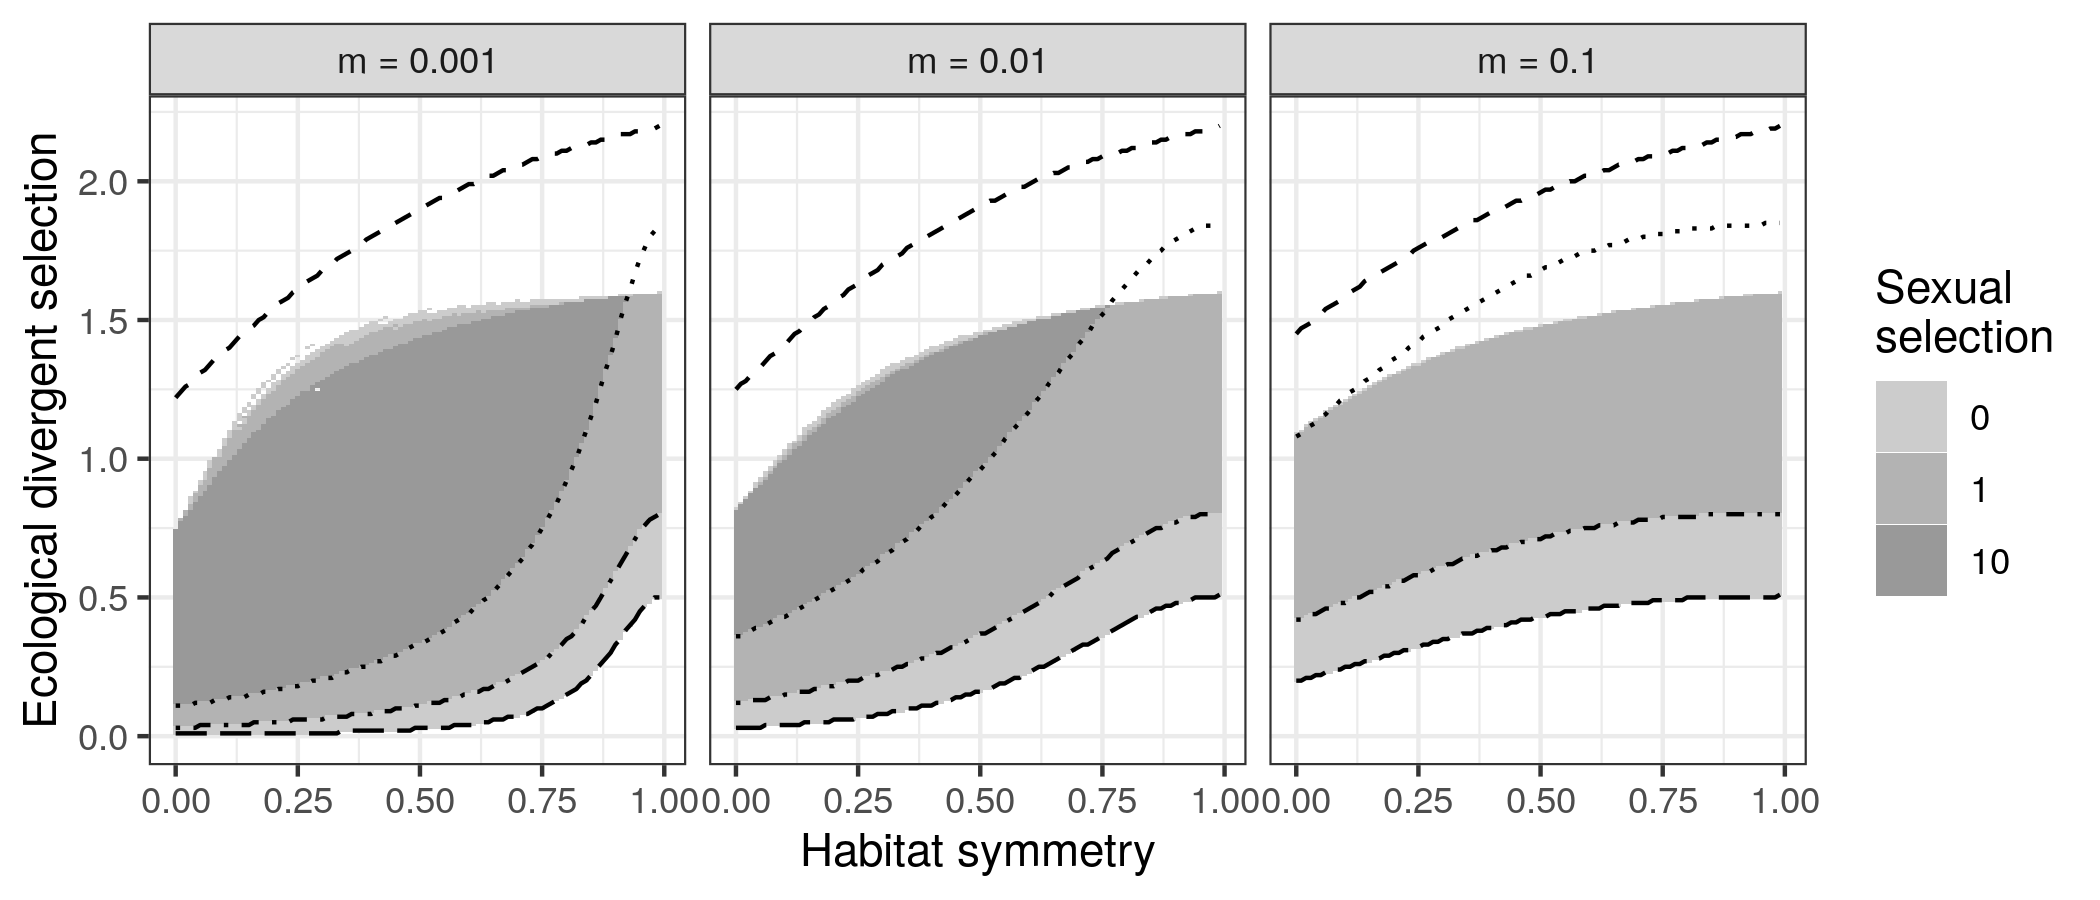
\includegraphics[width=\textwidth]{figures/map_branching_points}
    \caption{Branching throughout parameter space for three values of the dispersal rate $m$. Sexual selection increases the stability of evolutionary equilibria and therefore turns branching points into stable strategies. Shades of grey indicate the highest tested level $\alpha$ of sexual selection at which branching still occurs when a population is initially a specialist of the first resource ($x = -1$). Dashed lines expand the borders of the grey areas to show the full extent of where branching can theoretically occur, irrespective of the starting trait value.}
    \label{fig:map_branching_points}
\end{figure}

\begin{figure}
    \centering
    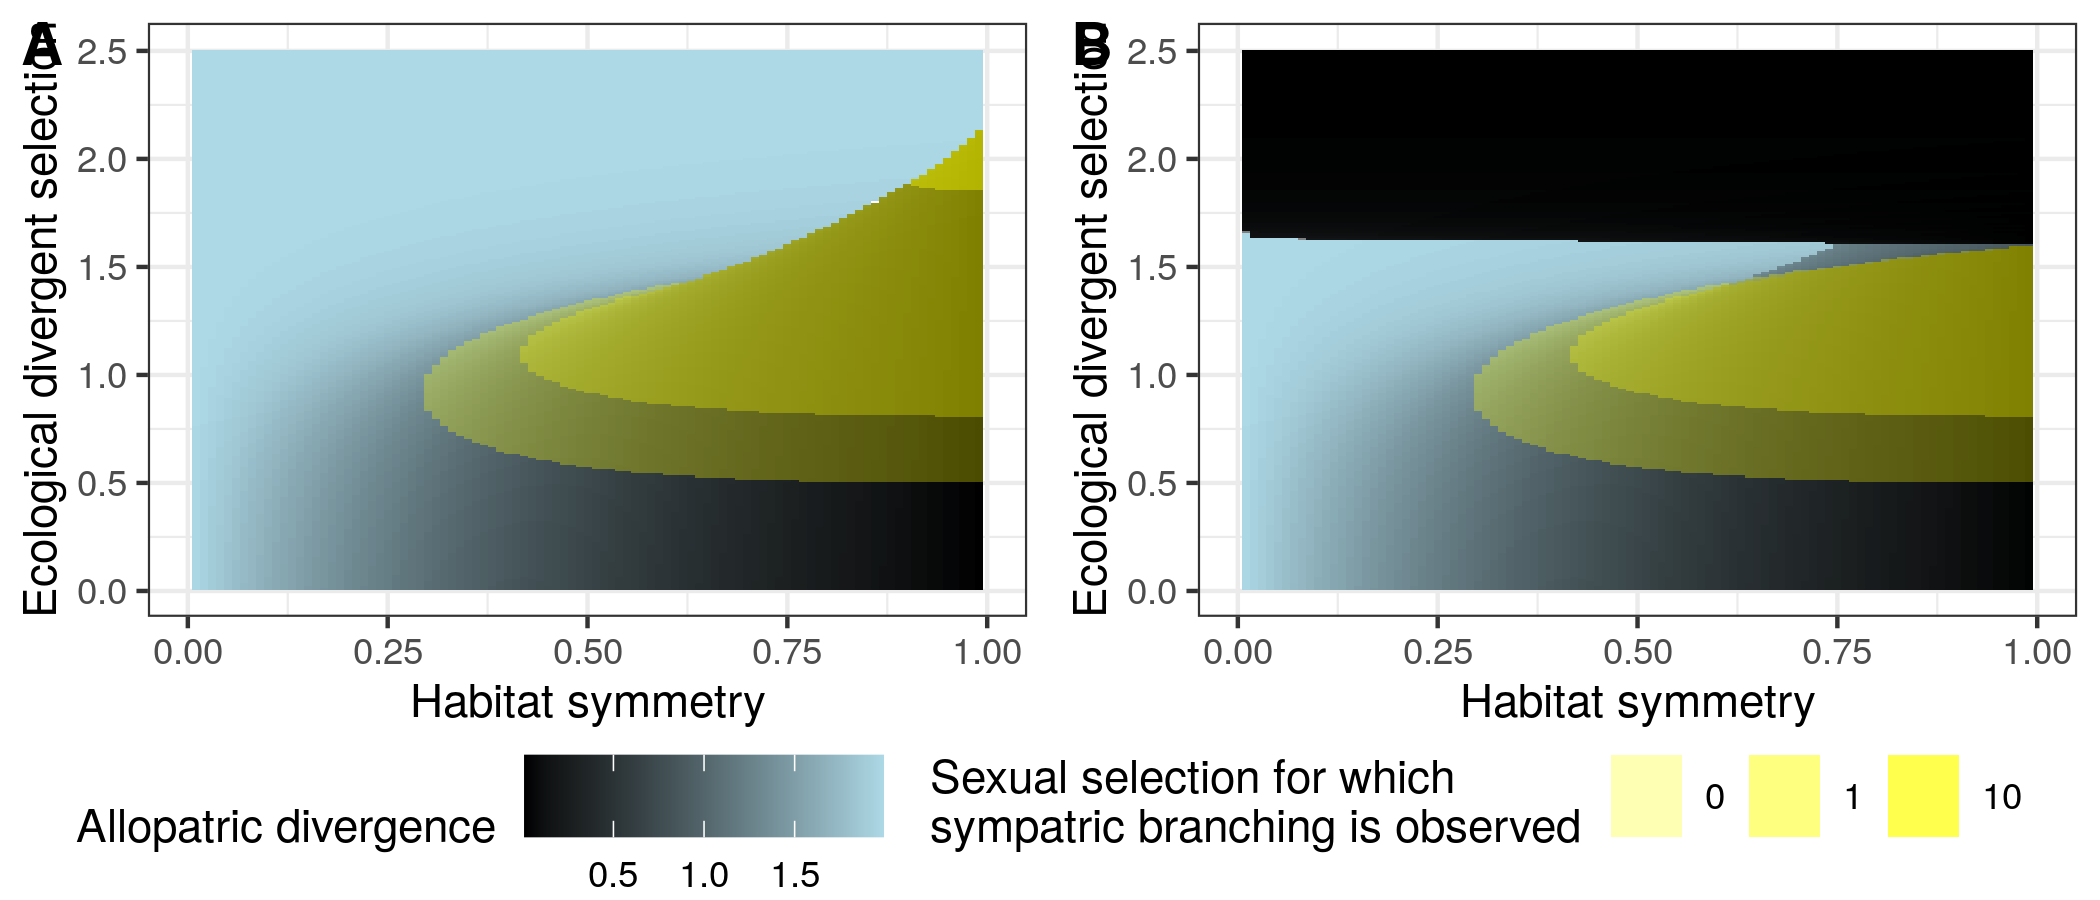
\includegraphics[width=\textwidth]{figures/divergence_across_patches}
    \caption{Adaptive dynamics of a model without dispersal, for two different starting points. In the absence of dispersal, one can disentangle the effect of local adaptation, i.e. the divergence in equilibrium trait value that occurs in allopatry (shades of blue), and competition, i.e. whether branching occurs in sympatry, within each patch (yellow transparent layer). Starting trait values: (A) $x = 0$, (B), $x = -1$.}
    \label{fig:map_divergence}
\end{figure}